
%% 
%% Copyright 2007, 2008, 2009 Elsevier Ltd
%% 
%% This file is part of the 'Elsarticle Bundle'.
%% ---------------------------------------------
%% 
%% It may be distributed under the conditions of the LaTeX Project Public
%% License, either version 1.2 of this license or (at your option) any
%% later version.  The latest version of this license is in
%%    http://www.latex-project.org/lppl.txt
%% and version 1.2 or later is part of all distributions of LaTeX
%% version 1999/12/01 or later.
%% 
%% The list of all files belonging to the 'Elsarticle Bundle' is
%% given in the file `manifest.txt'.
%% 
%% Template article for Elsevier's document class `elsarticle'
%% with harvard style bibliographic references
%% SP 2008/03/01

%% Use the option review to obtain double line spacing
\documentclass[authoryear,preprint,final,12pt]{elsarticle}

%%\documentclass[preprint,1p,authoryear]{elsarticle}
%\def\bibsection{\section*{References}}

%% Use the option review to obtain double line spacing
%% \documentclass[authoryear,preprint,review,12pt]{elsarticle}

%% Use the options 1p,twocolumn; 3p; 3p,twocolumn; 5p; or 5p,twocolumn
%% for a journal layout:
%% \documentclass[final,1p,times,authoryear]{elsarticle}
%% \documentclass[final,1p,times,twocolumn,authoryear]{elsarticle}
%% \documentclass[final,3p,times,authoryear]{elsarticle}
%% \documentclass[final,3p,times,twocolumn,authoryear]{elsarticle}
%% \documentclass[final,5p,times,authoryear]{elsarticle}
%% \documentclass[final,5p,times,twocolumn,authoryear]{elsarticle}

%% For including figures, graphicx.sty has been loaded in
%% elsarticle.cls. If you prefer to use the old commands
%% please give \usepackage{epsfig}

%% The amssymb package provides various useful mathematical symbols
\usepackage{floatrow}
%\usepackage{epstopdf}
\usepackage{amssymb}
\usepackage{multirow}
%\usepackage{subfigure}
\usepackage{array}
\usepackage{amsmath}
\usepackage{epsfig}

%\usepackage{apacite}
\usepackage{natbib}
\usepackage{algorithm}
\usepackage[noend]{algpseudocode}
\usepackage{csquotes}
%\usepackage{algorithmic}
\usepackage{hyperref}
\usepackage{verbatim}
%% The amsthm package provides extended theorem environments
%% \usepackage{amsthm}

%% The lineno packages adds line numbers. Start line numbering with
%% \begin{linenumbers}, end it with \end{linenumbers}. Or switch it on
%% for the whole article with \linenumbers.
%% \usepackage{lineno}
\usepackage[backend=biber,sorting=ynt]{biblatex}
 
\addbibresource{DB-p1-report.bib}

\journal{Database Systems}

\begin{document}

\begin{frontmatter}

%% Title, authors and addresses

%% use the tnoteref command within \title for footnotes;
%% use the tnotetext command for theassociated footnote;
%% use the fnref command within \author or \address for footnotes;
%% use the fntext command for theassociated footnote;
%% use the corref command within \author for corresponding author footnotes;
%% use the cortext command for theassociated footnote;
%% use the ead command for the email address,
%% and the form \ead[url] for the home page:

%% \title{Title\tnoteref{label1}}
%% \tnotetext[label1]{}
%% \author{Name\corref{cor1}\fnref{label2}}
%% \ead{email address}
%% \ead[url]{home page}
%% \fntext[label2]{}
%% \cortext[cor1]{}
%% \address{Address\fnref{label3}}
%% \fntext[label3]{}

\title{Professor Search Engine - Database Design Project 1}

%% use optional labels to link authors explicitly to addresses:
%% \author[label1,label2]{}
%% \address[label1]{}
%% \address[label2]{}

\author{Ya Wang - UIN: }
\ead{tonybest@tamu.edu}

\author{Yingyezhe Jin - UIN: 223001727}
\ead{jyyz@tamu.edu}

\cortext[cor1]{Corresponding author.}

\address{Department of Electrical and Computer Engineering,\\
Texas A\&M University,
College Station, TX 77843, United States}

\begin{abstract}
%% Text of abstract
This report presents a summary of the design of our professor information search engine. This information search engine enables the students to search faculty by their names and department and research areas and publications. The basic contact information and academic information of the professor is provided as the search result. We use Python to write a web crawler to retrieve the data of College of Engineering. We design the front-end website using PHP and Javascript. We built this system from scratch and learned in terms of SQL, Python, PHP and Javascript.
\end{abstract}

\begin{keyword}
%% keywords here, in the form: keyword \sep keyword
professor information search\sep database design
%% PACS codes here, in the form: \PACS code \sep code

%% MSC codes here, in the form: \MSC code \sep code
%% or \MSC[2008] code \sep code (2000 is the default)

\end{keyword}

\end{frontmatter}

%% \linenumbers

\section{Introduction}
% no \IEEEPARstart
For almost every university in the United State, there are certain websites for displaying their faculty information. But there is no such dedicated search engine in the university that can tell you those professors who focusing on certain given research areas. For example, if students want to see which professors are working the computer architecture, they might have to see the profile of each professor in the Computer Science department, which can waste them a lot of time. 

It is necessary for the universities to have the dedicated system for searching the  professors' information. On one hand, for both current and perspective students, it is desirable to have a website for searching the basic information (e.g. email, office, and personal website) of a professor, so that they can easily access the information and contact the professor. For other students who are interesting in finding an academic supervisor, they want to directly search the research areas and related publication of a professor without browsing through the personal website of the professor.

On the other hand, from the management point of view, the university officials need to have the access for editing the professors' information and be able to add or delete the contact and research information of those professors. Therefore, the professor search engine should also enable those basic operations on the database in the back-end. 

Given the requirements we discuss above, we should build a search engine that achieves:

1) Search the basic information including person contact and research information of the professors by name or department or their titles;

2) Search the research areas and publication information of the professor given the name of the professor or research area or publication title.

3) Enable the edition, deletion and insertion of the professor information. 

Practically, we design the search website as shown in Fig.~\ref{extract}. The website in Fig.~\ref{extract} is very intuitive and designed for daily use. We have also collected the needed data from the web and design the back-end database that supporting the search from scratch.

\begin{figure}[H]
\centering
 \includegraphics[width=3.5in]{figures/users-interfaces.eps}
 \caption{The Design of the searching website. (a) Search the professor basic and research information by name; (b) The display of the queried information with edition and deletion enabled.}
 \label{extract}
\end{figure}

The rest of the report is organized as follows: Section 2 briefly describes the data collection process and designed database schema. Section 3 introduces the functionality of our professor search engine. In Section 4, the learned experiences after finishing this project are listed. Finally, Section 5 summarizes and concludes the report. 


\section{Data Collection and Database Schema}
\subsection{Data Retrieval From the Web}
For the interest of this project itself and because of the limited time and scope, we only collect the professors' information in the \href{http://engineering.tamu.edu/academics/departments}{College of Engineering}, Texas A\&M University. A python web crawler is written for collecting the basic faculty information in department (Fig.~\ref{data}(a)). And for each faculty member, the crawler will also go the secondary link of that professor and obtain the detailed personal and research information including personal website, Google Scholar page, personal resume, research areas and publications (shown in Fig.~\ref{data}(b)). With the help of the widely used python library BeautifulSoup~\cite{bs}, we write the python web crawler to parse the structured HTML source code and extract the information needed for our professor search engine system. The python code can be found in the file named ``raw\_data/web\_crawler.py''.

\begin{figure}[H]
\centering
 \includegraphics[width=3in]{figures/data.eps}
 \caption{The faculty website of College of Engineering. (a) Extract the general professor information (e.g., email, office, and title); (b) Extract the personal and research information (e.g. research interest, personal webpage, curriculum vitae, and Google Scholar page) in the secondary link.}
 \label{data}
\end{figure}

\subsection{Database Schema Design}
The information collected from crawling the data in the university faculty website can be divided in four tables, namely ``basic information table'', ``academic information table'', ``research area table'', and ``publication table'' (shown in Fig.~\ref{tables}). Table~\ref{turple} illustrates the total number of turples in each table. %As shown in Fig.~\ref{data}(a), the basic information of each professor is one row of the basic table and each professor has his/her unique id in this table. Similarly, the academic information of each professor takes up to one row in academic table (shown in Fig.~\ref{data}(b)). And the research area and publication information of each professor is in research area and publication table (shown in Fig.~\ref{data}(c,d)). 

\begin{figure}[H]
\centering
 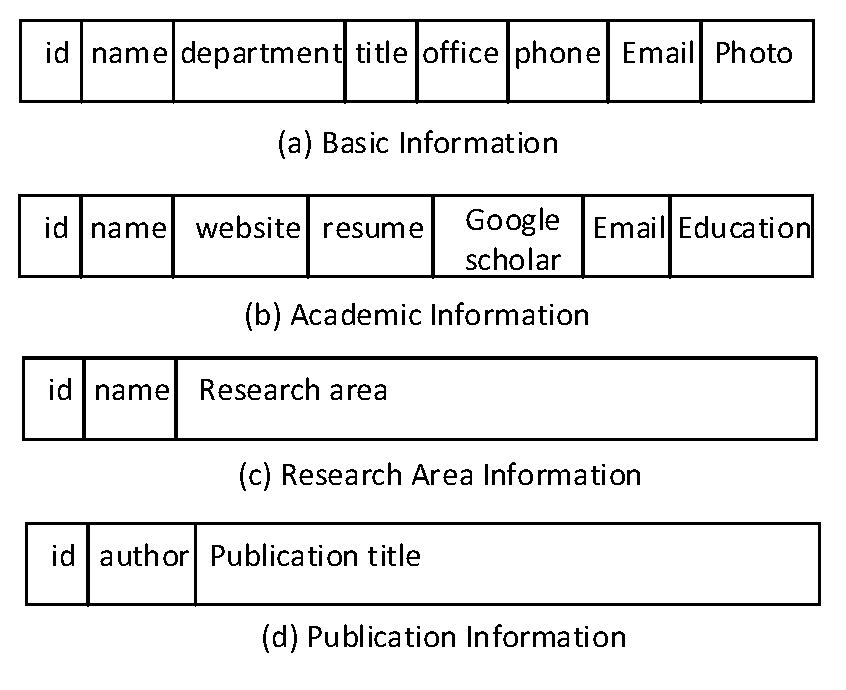
\includegraphics[width=3in]{figures/schema.eps}
 \caption{The schema of four tables.}
 \label{tables}
\end{figure}

\begin{table}[ht]
\caption{Total Turples in Each Table.}
\label{turple}
\begin{center}
\begin{tabular}{|l|c|}
\hline
Table Name					  &\# of Turples \\\cline{1-2}
Basic Information	      	  &  467	\\\cline{1-2}
Academic Information	      &  467	\\\cline{1-2}
Research Area Information	  &  1792	\\\cline{1-2}
Publication Information	      &  2196	\\\cline{1-2}
\hline
\end{tabular}
\end{center}
\end{table} 

We also attach our schema for creating the mySQL database in the file named ``schema.txt''.
%\verbatiminput{schema.txt}
In terms of handling the deletion where one turple references to turples in the other table (e.g. the professor name is used in all the tables), we intended to create a on-delete trigger to handle the deletion of one professor. But we do not have the permission to create the trigger in the CS cluster. Therefore, we handle it explicitly in the front-end when processing the SQL query.


\section{Web Application and Its Components}

There are two main functionalities of out web application. The first function is searching information from different tables in the database with keywords in a certain fields. The other function is performing data manipulation including add, edit and delete. For better presentation we also enabled pagination of the table results using features from mysql. The basic flowchart of our web applicaiton is shown in Fig. \ref{fig:1}.

\begin{figure}[h]
\centering
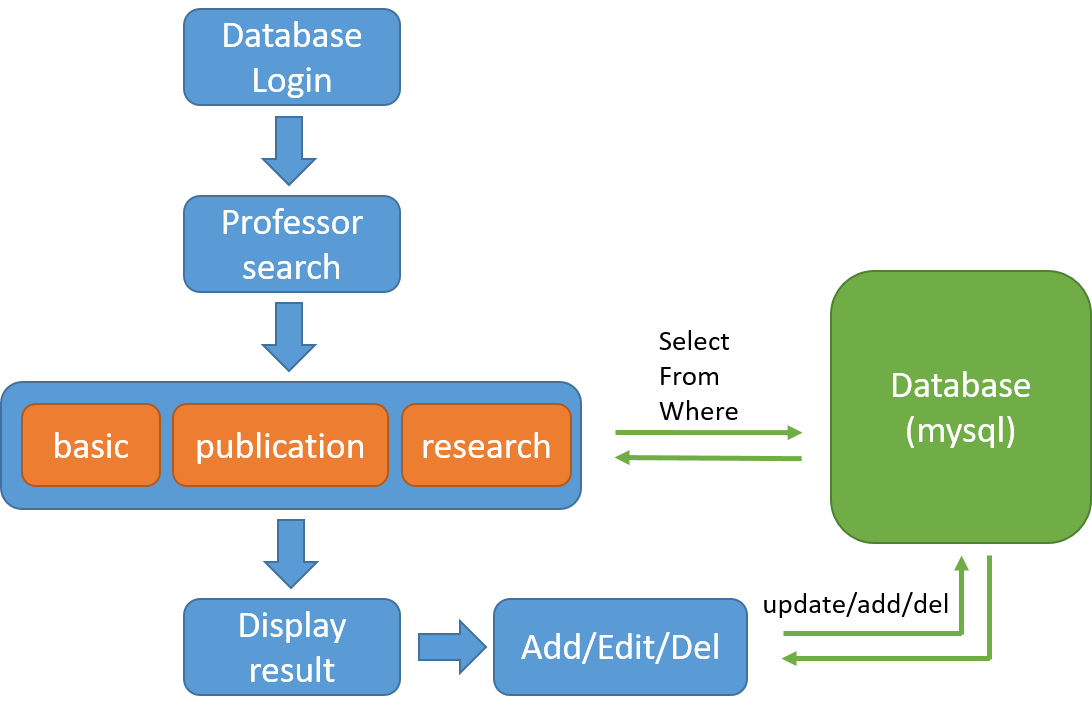
\includegraphics[width=5.0in]{flowchart.png}
\caption{The web application flowchart and interactions with database}
\label{fig:1}
\end{figure}

\subsection{Data Search}
There are three different search functions in our web application "Professor Search Engine". The first allows the user to search for basic information about professors. The user can look up for a professor's information using keyword "Faculty Name", "Department" and "Title". The information displayed in the search results are from two different tables, "basic table" and "academic table". The mysql query we choose to use is 
\begin{displayquote}
    SELECT basic.*, academic.website, academic.resume, academic.scholar, academic.education FROM basic, academic WHERE basic.name like \$name AND dept like \$dept AND title like \$title AND basic.name = academic.name 
\end{displayquote}
This allows the user to validly query two tables with keywords that only exists in one table. The results of the query is a new view that combines content from both tables. 

We also optimize the way to display the data obtained from query. From the query statement it can be seen that we are interested in four attributes "website", "resume", "scholar" and "education" from the "academic" table. We put "eduction" as a separate column in the search result we display. But for the other three which are just hyperlinks, we put them all under the name of the professor in each row. Thus the user can have a very clear view of all the information and know the link under names goes to corresponding resume/webstie/Google scholar of each professor.

The second search function allows user to search for publication titles and which professor published that paper. The table displayed for this search include the title of the publication and some simple information about the author including photo, name and department. To realize this functionality, we use the following query statement:
\begin{displayquote}
    SELECT publication.id, publication.author, basic.dept, basic.photo, publication.author, academic.name, academic.website, academic.resume, academic.scholar, publication.paper FROM basic, academic, publication WHERE basic.name like \$name AND basic.dept like \$dept AND publication.paper like \$ptitle AND basic.name = publication.author AND basic.name = academic.name 
\end{displayquote}
This also involves searching in three tables "basic table", "academic table" and "publication table" and stitching the returned column into one single view.

The last search function searches for research areas and related professor information. The table displayed for this search includes the specific area of research and the matched professor information including photo, name, department and email. The mysql query we used for this search is 
\begin{displayquote}
    SELECT research.id, basic.name, basic.dept, basic.email, basic.photo, research.name, academic.website, academic.resume, academic.scholar, research.area FROM basic, academic, research WHERE basic.name like \$name AND basic.dept like \$dept AND research.area like \$area AND basic.name = research.name AND basic.name = academic.name 
\end{displayquote}
This also involves searching in three tables "basic table", "academic table" and "publication table" and stitching the returned column into one single view.

All the text search field does not require exact match of the key words since we use like in mysql query. This way the user can exploit the full potential of the database.

\subsection{Data Manipulation}
In all three search functions, every row in the results is provided a link for user to edit/delete the information, thus providing the path for user to update the database. Clicking the delete link will directly result in the deletion of corresponding row in database. Clicking edit will result in a redirection to a new page where the user can edit each attributes of this row. Some rows are prohibited from editing, e.g. ID and name since these are related to natural joins between tables and thus sensitive to errors.

Since the search results are from different tables, editing the information will cause each attributes send back to its corresponding table with an UPDATE query statement.

\subsection{Pagination}
In order for a clear presentation of the table, we use pagination for each table display. Usually pagination is done by javascript on the client side since there are many well-developed framework to used (bootstrap, etc.). However we find a way to realize pagination using mysql keywords "LIMIT" without using any javacript. The trick is to add a "LIMIT start, size" to the end of each "SELECT FROM WHERE" statement made by the search engine. This will ask mysql to return the result from row "start" to row "start+size". Then each time the user click "Next" or "Previous", the server will increase/decrease the "start" by amount of "size", so mysql returns the correct information.

\section{Learn By Practicing}
This is an very interesting project, we have learned a lot of things. Before doing the project, we have little knowledge about Python and PHP and mySQL. But it turns out that we can quickly pick up those knowledge on the fly by Googling online documents and Stack overflow.

\section{Libraries and Tools}
Here is a list of external libraries and tool we used while developing the web application:
\begin{itemize}
    \item W3CSS\cite{w3css}: CSS format for web application.
    \item design1online\cite{design1onlinecom}: mysql based pagination. 
\end{itemize}
\section{Conclusion}
This project we start from collecting data using web crawler, then we design the web application for user to search/edit the professor information in database. Basic mysql operations are performed which gives us a chance to get familiarized with database, which helps us to understand the course and better prepares us for the second project.

% conference papers do not normally have an appendix


% use section* for acknowledgement
%\section*{Acknowledgment}


%The authors would like to thank...





% trigger a \newpage just before the given reference
% number - used to balance the columns on the last page
% adjust value as needed - may need to be readjusted if
% the document is modified later
%\IEEEtriggeratref{8}
% The "triggered" command can be changed if desired:
%\IEEEtriggercmd{\enlargethispage{-5in}}

% references section

% can use a bibliography generated by BibTeX as a .bbl file
% BibTeX documentation can be easily obtained at:
% http://www.ctan.org/tex-archive/biblio/bibtex/contrib/doc/
% The IEEEtran BibTeX style support page is at:
% http://www.michaelshell.org/tex/ieeetran/bibtex/
%\bibliographystyle{IEEEtran}
% argument is your BibTeX string definitions and bibliography database(s)
%\bibliography{IEEEabrv,../bib/paper}
%
% <OR> manually copy in the resultant .bbl file
% set second argument of \begin to the number of references
% (used to reserve space for the reference number labels box)

%% main text
%\section{}
%\label{}

%% The Appendices part is started with the command \appendix;
%% appendix sections are then done as normal sections
%% \appendix

%% \section{}
%% \label{}

%% If you have bibdatabase file and want bibtex to generate the
%% bibitems, please use
%%\
%%  \bibliographystyle{model5-names} 
\printbibliography
%% else use the following coding to input the bibitems directly in the
%% TeX file.

%\begin{thebibliography}{00}
% \bibitem[Author(year)]{label}
% Text of bibliographic item

%\bibitem[ ()]{}

%\end{thebibliography}
\end{document}

\endinput
%%
%% End of file `elsarticle-template-harv.tex'.
